% Paper 1, Mechanical Systems and Signal Processing. Elsevier CAS single-column template (cas-sc).
% Build: `make -C paper` (regenerates tables and number macros from results/, then LaTeX).
% Every number in the text is a macro from generated/numbers.tex or a table from tables/;
% none is typed by hand. Submission folder: `make -C paper submission`.
\documentclass[a4paper,fleqn]{cas-sc}
\usepackage[numbers,square,compress]{natbib}
\usepackage{bm,graphicx,longtable,booktabs}
\usepackage{lineno}
% Zenodo DOI of the archived release: fill in once, used by the data availability statement and the cover letter.
\providecommand{\ZenodoDOI}{[ZENODO DOI]}
  % \ZenodoDOI: the single place to fill in the archive DOI
\graphicspath{{figures/}{../figures/}}
\IfFileExists{tables/table1_parameters.tex}{\def\tabdir{tables}}{\def\tabdir{../results/tables}}
\newcommand{\inputtable}[1]{\input{\tabdir/#1}}

% generated by experiments/make_paper_numbers.py from results/ and config/; do not edit
\providecommand{\missing}[1]{\textbf{[missing: \texttt{#1}]}}
\newcommand{\AxleboxMass}{100}
\newcommand{\AxleboxModeContactHz}{1404}
\newcommand{\AxleboxModeNomHz}{503}
\newcommand{\BDBaseFortyBias}{0.277}
\newcommand{\BDBaseFortyRatio}{1.83}
\newcommand{\BDBaseSixtyBias}{0.284}
\newcommand{\BDBaseSixtyRatio}{1.87}
\newcommand{\BDExactBias}{0.274}
\newcommand{\BDExactRatio}{1.81}
\newcommand{\BDKFourBias}{0.239}
\newcommand{\BDKFourRatio}{1.76}
\newcommand{\BDKOneBias}{0.046}
\newcommand{\BDKOneRatio}{5.22}
\newcommand{\BDMaxDiffExact}{0.01}
\newcommand{\BDMaxDiffSNR}{0.02}
\newcommand{\BDSFtwoFortyBias}{0.021}
\newcommand{\BDSFtwoFortyRatio}{1.33}
\newcommand{\BDWideBias}{0.219}
\newcommand{\BDWideRatio}{1.53}
\newcommand{\BRegP}{0.049}
\newcommand{\BRegPayloadP}{0.042}
\newcommand{\BRegRsq}{0.19}
\newcommand{\BudgetCoest}{3.9}
\newcommand{\BudgetCoestMassOne}{1.8}
\newcommand{\BudgetNominal}{6.1}
\newcommand{\BudgetNominalMassOne}{5.1}
\newcommand{\CalBiasForty}{0.09}
\newcommand{\CalInflForty}{1.39}
\newcommand{\CalSlope}{0.99998}
\newcommand{\CalSplitACov}{0.80}
\newcommand{\CalSplitAHi}{0.94}
\newcommand{\CalSplitAInfl}{1.32}
\newcommand{\CalSplitALo}{0.56}
\newcommand{\CalSplitAk}{16}
\newcommand{\CalSplitAn}{20}
\newcommand{\CalSplitBCov}{0.97}
\newcommand{\CalSplitBHi}{1.00}
\newcommand{\CalSplitBInfl}{1.48}
\newcommand{\CalSplitBLo}{0.83}
\newcommand{\CalSplitBk}{29}
\newcommand{\CalSplitBn}{30}
\newcommand{\CalTwentyRawCov}{0.90}
\newcommand{\ClearanceZero}{20}
\newcommand{\ContactPctTenEmpty}{-6.2}
\newcommand{\ContactPctTenLoaded}{-2.0}
\newcommand{\DebiasBin}{0.47}
\newcommand{\DebiasDeb}{0.07}
\newcommand{\DebiasNoise}{0.06}
\newcommand{\DebiasRecords}{300}
\newcommand{\DilutionEmpty}{0.17}
\newcommand{\DilutionLoaded}{0.13}
\newcommand{\DriftCoestMDC}{0.71}
\newcommand{\DriftMCCoestFA}{1}
\newcommand{\DriftMCCoestHi}{0.25}
\newcommand{\DriftMCCoestLo}{0.00}
\newcommand{\DriftMCCoestMean}{-0.02}
\newcommand{\DriftMCCoestN}{20}
\newcommand{\DriftMCNomFA}{20}
\newcommand{\DriftMCNomHi}{1.00}
\newcommand{\DriftMCNomLo}{0.83}
\newcommand{\DriftMCNomMean}{-2.21}
\newcommand{\DriftMCNomN}{20}
\newcommand{\DriftSoftTenApparent}{-0.67}
\newcommand{\DriftSoftTenFA}{0.87}
\newcommand{\DriftSoftTwentyApparent}{-2.03}
\newcommand{\DriftStiffTenMDC}{1.2}
\newcommand{\DriftStiffTwentyMDC}{1.8}
\newcommand{\EffPctTenEmpty}{-1.1}
\newcommand{\EffPctTenLoaded}{-0.26}
\newcommand{\ExpCRBFifty}{0.0034}
\newcommand{\ExpCRBTwoHundred}{0.0019}
\newcommand{\ExpMDCFifty}{0.0141}
\newcommand{\ExpMDCTwoHundred}{0.0077}
\newcommand{\ExpShiftTen}{0.0053}
\newcommand{\ExpShiftTwenty}{0.0097}
\newcommand{\GyroRatio}{0.10}
\newcommand{\HLFortyBias}{0.09}
\newcommand{\HLFortyBiasSE}{0.03}
\newcommand{\HLFortyCRB}{0.17}
\newcommand{\HLFortyCov}{0.76}
\newcommand{\HLFortyCovHi}{0.87}
\newcommand{\HLFortyCovLo}{0.62}
\newcommand{\HLFortyRMSE}{0.24}
\newcommand{\HLFortyRatioCRB}{1.39}
\newcommand{\HLFortyRatioSE}{1.39}
\newcommand{\HLFortycBBias}{7.1}
\newcommand{\HLN}{50}
\newcommand{\HLTwentyBias}{0.10}
\newcommand{\HLTwentyBiasSE}{0.02}
\newcommand{\HLTwentyCRB}{0.18}
\newcommand{\HLTwentyCov}{0.90}
\newcommand{\HLTwentyCovHi}{0.97}
\newcommand{\HLTwentyCovLo}{0.78}
\newcommand{\HLTwentyRMSE}{0.19}
\newcommand{\HLTwentyRatioCRB}{1.09}
\newcommand{\HLTwentyRatioSE}{1.08}
\newcommand{\HLTwentycBBias}{3.0}
\newcommand{\ICDiffMean}{\missing{p4/inverse_crime.json}}
\newcommand{\ICNLBias}{\missing{p4/inverse_crime.json}}
\newcommand{\ICNLCovCal}{\missing{p4/inverse_crime.json}}
\newcommand{\ICNLN}{\missing{p4/inverse_crime.json}}
\newcommand{\ICNLRMSE}{\missing{p4/inverse_crime.json}}
\newcommand{\ICPairsFACal}{\missing{p4/inverse_crime.json}}
\newcommand{\ICPairsN}{\missing{p4/inverse_crime.json}}
\newcommand{\IgnoreCouplingForty}{-14.0}
\newcommand{\IgnoreCouplingTwenty}{-13.9}
\newcommand{\KBCRBExpFixed}{0.17}
\newcommand{\KBCRBExpFree}{0.26}
\newcommand{\KapCalCovered}{14}
\newcommand{\KapCalHi}{0.88}
\newcommand{\KapCalLo}{0.46}
\newcommand{\KapCalN}{20}
\newcommand{\KapCoestCovered}{14}
\newcommand{\KapCoestHi}{0.88}
\newcommand{\KapCoestKfMax}{2.19}
\newcommand{\KapCoestKfMin}{0.58}
\newcommand{\KapCoestLo}{0.46}
\newcommand{\KapCoestMean}{0.057}
\newcommand{\KapCoestN}{20}
\newcommand{\KapCoestRMS}{0.096}
\newcommand{\KapNomCov}{0.70}
\newcommand{\KapNomGainErr}{0.42}
\newcommand{\KapNomHi}{0.88}
\newcommand{\KapNomLo}{0.46}
\newcommand{\KapNomN}{20}
\newcommand{\KappaCoest}{0.044}
\newcommand{\KappaKfTerm}{0.24}
\newcommand{\KappaNominal}{0.26}
\newcommand{\KcontactEmpty}{5.9}
\newcommand{\KcontactLoaded}{7.8}
\newcommand{\KernelFine}{4}
\newcommand{\KernelHalfWidth}{120}
\newcommand{\LoadExp}{0.1}
\newcommand{\MDCCalFiftyForty}{1.00}
\newcommand{\MDCCalFiftyTwenty}{0.71}
\newcommand{\MDCCalTwoHundredForty}{0.48}
\newcommand{\MDCCalTwoHundredTwenty}{0.36}
\newcommand{\MDCFiftyForty}{0.72}
\newcommand{\MDCFiftyTwenty}{0.71}
\newcommand{\MDCTwoHundredForty}{0.34}
\newcommand{\MDCTwoHundredTwenty}{0.36}
\newcommand{\MWCRBFixedMax}{0.88}
\newcommand{\MWCRBFixedMin}{0.76}
\newcommand{\MWCRBMax}{0.17}
\newcommand{\MWCRBMin}{0.16}
\newcommand{\MWCorrectBiasEight}{0.04}
\newcommand{\MWCorrectBiasFour}{0.12}
\newcommand{\MWCorrectBiasSEEight}{0.04}
\newcommand{\MWCorrectBiasSEFour}{0.04}
\newcommand{\MWCorrectBiasSETwo}{0.07}
\newcommand{\MWCorrectBiasTwo}{0.24}
\newcommand{\MWSingleBiasEight}{-8.6}
\newcommand{\MWSingleBiasFour}{-13.9}
\newcommand{\MWSingleBiasTwo}{-13.3}
\newcommand{\NElements}{32}
\newcommand{\NumRevs}{20}
\newcommand{\PCBiasMax}{0.09}
\newcommand{\PCModelRatioMax}{0.82}
\newcommand{\PCModelRatioMin}{0.64}
\newcommand{\PCSandRatioMax}{1.10}
\newcommand{\PCSandRatioMin}{1.08}
\newcommand{\PTwoCTMedianCorr}{9.36}
\newcommand{\PTwoCTOutsideClean}{11}
\newcommand{\PTwoCTOutsideCorr}{46}
\newcommand{\PTwoWhCovClean}{0.80}
\newcommand{\PTwoWhCovCorr}{0.45}
\newcommand{\PTwoWhMedianClean}{7.71}
\newcommand{\PTwoWhMedianCorr}{7.74}
\newcommand{\PayloadMax}{22.5}
\newcommand{\PayloadMin}{5.5}
\newcommand{\PeffSeries}{0.027}
\newcommand{\RSEBlockCovForty}{0.74}
\newcommand{\RSEBlockSEForty}{0.179}
\newcommand{\RSEModelCovForty}{0.68}
\newcommand{\RSEModelSEForty}{0.170}
\newcommand{\RollersPerRow}{21}
\newcommand{\SensKf}{0.60}
\newcommand{\SensUnsprung}{-12.1}
\newcommand{\SpeedCRBFixed}{0.66}
\newcommand{\SpeedCRBNarrow}{0.47}
\newcommand{\SpeedCRBWide}{0.23}
\newcommand{\SpeedCRBWideTwoHundred}{0.11}
\newcommand{\SweepCRBMax}{\missing{p4/sweep.json}}
\newcommand{\SweepCRBMin}{\missing{p4/sweep.json}}
\newcommand{\SweepMDCMax}{\missing{p4/sweep.json}}
\newcommand{\SweepMDCMin}{\missing{p4/sweep.json}}
\newcommand{\SweepModeMax}{\missing{p4/sweep.json}}
\newcommand{\SweepModeMin}{\missing{p4/sweep.json}}
\newcommand{\SweepNomCRB}{\missing{p4/sweep.json}}
\newcommand{\SweepNomMDC}{\missing{p4/sweep.json}}
\newcommand{\SweepNomMode}{\missing{p4/sweep.json}}
\newcommand{\WIMsigmaPct}{3}
\newcommand{\WLNone}{0.23}
\newcommand{\WLNotchCost}{2}
\newcommand{\WLTachoTen}{0.10}
\newcommand{\WLTachoZero}{0.18}
\newcommand{\kBnom}{1}


\begin{document}
\let\WriteBookmarks\relax
\def\floatpagepagefraction{1}
\def\textpagefraction{.001}

\shorttitle{Support stiffness of wheelset bearings from axle-box acceleration}
% Authors, affiliations and the corresponding author: to be completed by the authors before submission.
\author[aff1]{Author One\corref{cor1}}
\ead{corresponding.author@institution.example}
\cortext[cor1]{Corresponding author.}
\affiliation[aff1]{organization={Institution},
            city={City},
            country={Country}}


\title[mode=title]{Tracking the support stiffness of railway wheelset bearings from multi-speed
axle-box acceleration without measuring rail roughness: a multi-pass debiased Whittle likelihood}

\begin{abstract}
Loss of the vertical support stiffness of a wheelset bearing, through loose fits, a degraded housing,
adapter or pad, or clearance growth, shifts the resonance of the axlebox on its support. On freight
wagons this resonance lies in the band of axle-box acceleration excited by rail roughness, so a
stiffness identified from it is confounded with the unknown roughness. We pool passes at
different speeds and payloads in a single debiased Whittle likelihood: the resonance stays fixed in
frequency while the roughness excitation moves with speed, so the roughness levels can be left as free
nuisance parameters. A finite-element wheelset is coupled to neighbouring
wheels through an infinite Timoshenko rail. For a representative freight wagon (Y25 bogies, ballasted
60E1 track) and 50 passes at 60--110~km/h, simulations give a bias of at most \HLBiasAbsMax\% and a
root-mean-square error of \HLRMSEMin--\HLRMSEMax\%, within \HLRatioCRBMax{} times the Cram\'er--Rao
bound. Ignoring wheel-to-wheel coupling biases the estimate by \IgnoreCouplingForty\%; nonlinear
Hertzian contact shifts it by only \ICDiffMean{} percentage points. Because absolute values carry a
model-form uncertainty of about \BudgetCoest\%, the method targets changes between periods. With the
foundation and contact stiffness re-estimated in each period, a decrease of
\MDCCalFiftyMin--\MDCCalFiftyMax\% is detectable from 50 passes per period and
\MDCCalTwoHundredMin--\MDCCalTwoHundredMax\% from 200, and a 20\% softer foundation, which appears as a
\DriftSoftTwentyApparent\% change if the track is held fixed, causes no bias. Clearance growth changes the
effective stiffness little (\EffPctTenEmpty\% per 10~\textmu m), so the method reports support-stiffness
loss rather than its mechanism.
\end{abstract}


\begin{keywords}
axle-box acceleration \sep wheelset bearing support stiffness \sep condition monitoring \sep
debiased Whittle likelihood \sep rail roughness \sep vehicle--track interaction \sep system identification
\end{keywords}

\maketitle
\linenumbers

% Section 1: introduction, in the order required by the MSSP Guide for Authors: problem statement; state
% of the art by method family; motivation; principle of the approach; contributions; importance and
% impact. The novelty statement (second paragraph of the contributions part) is fixed wording (2026-10-15).
\section{Introduction}\label{sec:intro}

\paragraph{Problem statement.} Each journal of a railway wheelset carries the axle load into the
axlebox through the rollers of the bearing, the bearing housing, the adapter and, on many bogies, an
elastomeric pad. We call the vertical stiffness of this load path the effective support stiffness
$k_B$. It falls when the bearing fits loosen, when the housing, adapter or pad degrades, or when the
bearing clearance grows. The problem addressed here is to estimate $k_B$, and changes of it between
monitoring periods, from the vertical axle-box acceleration (ABA) of a wagon in normal service, when the
rail roughness that excites the response is not measured.

\paragraph{State of the art.} Four families of methods bear on this problem.
\emph{Bearing fault diagnostics} detect localised rolling-contact damage from the impacts it produces,
using envelope and spectral-kurtosis analysis of high-frequency vibration~\citep{randall2011}, or from
the bearing temperature. They are mature and need no model of the vehicle, but they respond to impacts
at roller-passing frequencies, not to a gradual loss of stiffness, so loose fits or a degraded pad
remain invisible until secondary damage occurs.
\emph{Model-based processing of ABA for the track} uses a vehicle--track model to turn ABA into rail
roughness or track stiffness. Roughness is estimated by inverse filtering or source identification
with a known vehicle transfer function~\citep{pieringer2022,carrigan2023}; track stiffness is estimated
from the P2 resonance of single passes~\citep{carrigan2023} or by matching a library of simulations,
where the irregularity level enters as one parameter~\citep{shen2023}. These methods use the known
vehicle as the instrument; they assume the vehicle parameters, and the targets lie below the
axle-box support band. Per-pass estimates also scatter widely when the roughness spectrum has features
near the resonance used~\citep{carrigan2023}.
\emph{Joint identification of vehicle parameters with unknown excitation} has been developed for road
vehicles, where the excitation is separated from the vehicle by the time lag between axles in a Kalman
filter with unknown input~\citep{liu2024}, by a Bayesian formulation in the frequency
domain~\citep{an2024}, or by modelling the road as a Gaussian random field~\citep{guo2026}. Railway
suspension parameters have been identified as a statistical inverse problem with a surrogate model,
using measured track irregularities as input~\citep{lebel2019,lebelhal}. These methods need either the
measured excitation or a model of its structure (time lag between axles, random field), and they have
been demonstrated for suspension parameters at low frequencies, well below the axle-box support band.
\emph{Output-only identification with an unknown excitation spectrum}, such as operational modal
analysis with a Bayesian FFT likelihood~\citep{au2011} or drive-by monitoring that removes road
roughness by subtracting responses recorded at different speeds~\citep{jin2021}, treats the excitation as a nuisance
in a frequency-domain likelihood. It is statistically efficient, but it assumes a smooth excitation
spectrum near each mode and, in its standard form, a single record, so it does not separate a vehicle
resonance from a roughness spectrum that is itself unknown and changes from pass to pass.

\paragraph{Closest work and literature search.} Table~\ref{tab:novelty} compares the method with the
closest work on axle-box acceleration~\citep{carrigan2023,shen2023,pieringer2022} and with axlebox
bearing-response models~\citep{li2019axlebox,guan2023}, which predict bearing loads and vibration for
a given excitation but do not identify the support. The search covered 11--16 October 2026 and used a
general web search engine; bibliographic databases (Scopus, Web of Science, Google Scholar) could not be
queried directly from the computing environment, and full texts were read where they were accessible,
otherwise abstracts. Search terms combined ``axle box acceleration'' or ``axlebox bearing'' with rail
roughness, track stiffness, bearing stiffness or support stiffness, identification, unknown excitation and
speed; further searches covered joint identification of vehicle parameters and road or track
irregularity, operational modal analysis with unknown excitation spectra, drive-by monitoring at several
speeds, and the debiased Whittle likelihood. No lower date limit was set. Only English-language sources
were searched; Chinese- and Japanese-language work on axlebox bearings was not covered.

\begin{table}[tbp]\centering\scriptsize
\caption{Comparison with the closest work. Entries for other work are taken from the cited papers as far as
they could be read (n.r.: not reported in the parts read).}\label{tab:novelty}
\resizebox{\textwidth}{!}{\begin{tabular}{p{2.2cm}p{2.0cm}p{2.1cm}p{1.8cm}p{2.1cm}p{1.6cm}p{2.0cm}p{1.9cm}p{1.9cm}}
\toprule
Work & Target parameter & Excitation assumption & Speed pooling & Roughness treatment & Wheel coupling &
Measurements needed & Validation type & Uncertainty calibration \\
\midrule
Pieringer and Kropp~\citep{pieringer2022} & Rail roughness & Contact force recovered from ABA; track dynamics known & No (single pass) & Estimated output, via a Hertzian contact model & n.r. & ABA, known track parameters & Simulation & Sensitivity to rail-pad stiffness; no intervals \\
Carrigan and Talbot~\citep{carrigan2023} & Track stiffness, then rail roughness & Unknown roughness, removed after the stiffness fit & No (per pass, along the track) & Deconvolution after a P2 peak fit & Several wheels on one rail & ABA, speed, wheel angle (comb filter) & Simulation and metro field trials & Per-pass scatter; no intervals \\
Shen et al.~\citep{shen2023} & Rail-pad and ballast stiffness, irregularity level & Irregularity as a single level parameter & No (three speeds estimated separately) & One level parameter & n.r. & ABA & n.r. & n.r. \\
Li et al.~\citep{li2019axlebox} & None (forward model of bearing loads) & Prescribed track irregularity & -- & Prescribed input & Vehicle model & -- & Wheelset test rig & -- \\
Guan et al.~\citep{guan2023} & None (forward model of bearing response) & Prescribed wheel polygon and irregularity & -- & Prescribed input & Flexible wheelset & -- & Simulation & -- \\
This paper & Bearing support stiffness $k_{B0}$ (and $c_B$) and its change & Unknown roughness, spectrum with free sub-band levels & Yes, many passes in one likelihood & Nuisance levels shared by a period, profiled & Neighbouring wheels via an infinite Timoshenko rail & ABA, speed, WIM payload, distance-aligned records & Matched-model simulation, with model-error and nonlinear-contact checks & CRB, Wald and profile intervals, simulation calibration, inflation for simultaneous model errors \\
\bottomrule
\end{tabular}}
\end{table}

\paragraph{Motivation.} The support resonance of a freight wheelset, the axlebox vibrating on its
support, lies at a few hundred hertz, inside the band in which ABA is excited by rail roughness. ABA is
already recorded in service for track monitoring, so the support stiffness could be tracked from data
that are collected anyway, without a dedicated test, provided the records meet requirements on bandwidth,
calibration, speed and record alignment (Section~\ref{sec:requirements}). None of the families above provides
this: fault diagnostics do not see stiffness, the track methods assume the vehicle, and the
joint-identification methods need the excitation or work below the support band. The work is
motivated by condition monitoring of freight wagons on Indian Railways. The vehicle and track values
that a model of an Indian wagon needs are not yet available to us and are pending data from the
Research Designs and Standards Organisation (RDSO). The method is therefore developed and assessed
here for a representative European freight wagon, a four-axle Eaos/Eanos-type wagon on Y25 bogies on
ballasted UIC60 track, for which the parameters are published; values that could not be found are swept
over plausible ranges.

\paragraph{Principle of the approach.} The support resonance is fixed in frequency, while the roughness
excitation is fixed in wavenumber and therefore moves in frequency with the train speed. Passes at
different speeds thus see the same resonance through different parts of the roughness spectrum. We pool
many passes in one frequency-domain likelihood in which the roughness level of each wavenumber sub-band
is a free nuisance parameter shared by all passes, payload enters through a weigh-in-motion measurement,
and the leakage of the finite records is handled by the debiased Whittle likelihood~\citep{sykulski2019}.
The forward model couples the instrumented wheelset to its neighbours through the rail, because the
other wheels of the bogie and wagon load the rail at the same time.

\paragraph{Contributions.}
To our knowledge, this is the first method to identify the vertical stiffness of the axle-box bearing
support from multi-speed axle-box acceleration without measuring rail roughness. The support resonance
and the roughness are separated by pooling passes at different speeds and payloads in a single
debiased Whittle likelihood, in which roughness levels are free nuisance parameters. Joint estimation
of vehicle or track parameters with unknown excitation has been studied for track stiffness
\citep{carrigan2023,shen2023} and for road-vehicle suspensions \citep{liu2024,an2024}. There, roughness
is handled by deconvolution, a single level parameter, or axle time lags, and the targets lie below the
axle-box support band. Specifically, this paper contributes:
\begin{enumerate}
\item a multi-pass debiased Whittle likelihood that identifies the effective support stiffness and
damping of a wheelset bearing from ABA spectra of many passes, with the roughness level of each
sub-band a free nuisance parameter and payload from a weigh-in-motion measurement;
\item a forward model in which the instrumented wheelset is coupled to its neighbours through an
infinite Timoshenko rail with the phase factors between wheels kept, and evidence that ignoring this
coupling biases the support stiffness by \IgnoreCouplingForty\%;
\item an uncertainty budget for a representative freight wagon, separating statistical error
(Cram\'er--Rao bounds, matched-model Monte Carlo bias and coverage), parameter error (model-form
sensitivity, sweeps over the published parameter ranges, simultaneous model errors), model-structure error
(nonlinear Hertzian contact, payload-dependent primary suspension, wheel coupling) and measurement and
operating conditions;
\item a procedure for detecting changes between monitoring periods that re-estimates the track
foundation and contact stiffness in each period, with detection limits (nominal and allowing for
simultaneous model errors), false-alarm rates under track drift, and the bearing clearance growth that
the detection limit corresponds to. Periods must be compared within one payload band (empty or laden):
pooling passes of mixed payload is not supported by the present model, because the primary suspension
changes with payload.
\end{enumerate}

\paragraph{Importance and impact.} A loss of support stiffness changes the load path of the bearing and
the dynamic loads on it, and it can develop without the temperature rise or impacts that existing
bearing monitoring detects. Detecting it from axle-box records that instrumented wagons already collect
would add a monitoring channel without new hardware on the wheelset. The statistical basis of the method
gives detection limits and false-alarm rates that can be stated in advance for a given monitoring
design. All results in this paper are from matched-model simulations, in which data and estimator share
the vehicle--track model apart from the deliberate perturbations studied; they establish the method and
its error budget, not its operational performance, which requires a controlled rig or field test with a
known change of support stiffness. The same likelihood applies to other vehicle--track resonances excited
by unmeasured roughness.

Section~\ref{sec:model} describes the vehicle--track model and Section~\ref{sec:method} the
estimator. Section~\ref{sec:results} verifies and demonstrates the method in simulation,
Section~\ref{sec:discussion} discusses the results and their limitations, and
Section~\ref{sec:conclusions} concludes.

% Section 2: model. Numbers: generated/numbers.tex; tables: ../results/tables/*.tex.
\section{Vehicle--track model}\label{sec:model}

\subsection{Wheelset and the effective support stiffness}\label{sec:wheelset}
The wheelset is a stepped Timoshenko beam (axle body, wheel seats, dust-guard collars and journals)
discretised with \NElements{} two-node elements with interdependent interpolation, which are free of
shear locking~\citep{friedman1993}. The shear coefficient is Cowper's value for a solid circular
section~\citep{cowper1966}. Each wheel is a rigid disc with mass and diametral inertia at its seat.
Each axlebox is a rigid mass on its journal, tied to a bogie frame that is held fixed by a linear
primary spring--damper pair. Axle damping is stiffness proportional. The model is linear and
vertical-plane. Gyroscopic and rotating-damping terms are omitted: the rotation rate is
\GyroRatio{} of the first constrained bending frequency at the reference speed (Table~\ref{tab:table2_verification}).

Between each journal and its axlebox the model has one spring--damper pair, $k_B$ and $c_B$. We call
$k_B$ the \emph{effective support stiffness}: the stiffness of the load path from journal to axlebox,
that is, the roller contacts of the bearing in series with the bearing housing, the adapter and any
pad,
\begin{equation}
  k_B(W, c) = \left[\frac{1}{k_\mathrm{contact}(W, c)} + \frac{1}{k_\mathrm{housing}}\right]^{-1},
  \label{eq:series}
\end{equation}
where $W$ is the axle load and $c$ the diametral clearance of the bearing. The quantity monitored in
this paper is a loss of $k_B$. It covers loosening of the bearing fits, degradation of the housing,
adapter or pad, and growth of the bearing clearance. It is not a model of rolling-contact fatigue
or spalling, which act at much higher frequencies through impacts.

\paragraph{Roller contacts.} For a double-row roller bearing under a static radial load, the
contact stiffness follows from the line-contact law of the wheelset model, $Q = K_n\,\delta^{10/9}$,
with the load shared over the rollers in the load zone (roller deflection
$\delta_j = \Delta\cos\theta_j\cos\alpha - c/2$, contact force summed over both rows; inner and
outer contacts in series; \citealp{harris2006}). For a generic freight unit
(placeholder geometry, \RollersPerRow{} rollers per row, initial clearance \ClearanceZero~\textmu m;
Table~\ref{tab:table1_parameters}) the cage-averaged contact stiffness is
\KcontactEmpty{} and \KcontactLoaded{}~GN/m per bearing at the empty and loaded axle loads.
These values are 6--8 times the nominal effective support stiffness of \kBnom~GN/m used throughout
(a placeholder), so in reading~\eqref{eq:series} the housing path carries most of the compliance.
A change of the contact stiffness then reaches $k_B$ diluted by the factor $k_B/k_\mathrm{contact}$,
\DilutionEmpty{} (empty) to \DilutionLoaded{} (loaded): a clearance growth of 10~\textmu m lowers the
contact stiffness by \ContactPctTenEmpty\% (empty) and \ContactPctTenLoaded\% (loaded), and $k_B$ by
\EffPctTenEmpty\% and \EffPctTenLoaded\%.

If instead $k_B$ were the contact stiffness alone, the axlebox-on-bearing resonance would sit near
\AxleboxModeContactHz~Hz (single-mass estimate with the \AxleboxMass~kg axlebox), where contact
filtering, the rail pinned--pinned mode and the flexible modes of the wheels, none of which the
model contains, dominate; that reading is outside the scope of this paper.

\paragraph{Load dependence.} The default stiffness law used for all results is the power law
\begin{equation}
  k_B(W) = k_{B0}\,(W/W_0)^{p},\qquad p = \LoadExp,
  \label{eq:powerlaw}
\end{equation}
the exponent of a line contact at zero clearance, with $W_0$ the loaded axle load and $k_{B0}$ the
health parameter. The series law~\eqref{eq:series}, with $k_\mathrm{housing}$ set so that
$k_B(W_0, c_0) = k_{B0}$, is implemented as an option; its effective exponent over the payload range
is \PeffSeries{}. The exponent is held fixed in the estimator; Section~\ref{sec:limitations}
discusses why it does not serve as a second, clearance-specific indicator.

\subsection{Rail, contact and multi-wheel coupling}\label{sec:rail}
The rail is an infinite Timoshenko beam on a continuous foundation of complex stiffness per unit
length $k_f(1+\mathrm{i}\eta_f)$. Its point and transfer receptances $R(x)$ follow in closed form by
partial fractions of the wavenumber-domain solution; the result equals Eq.~(11) of
Carrigan and Talbot~\citep{carrigan2023} and is checked against a numerical inverse transform. Rail
and foundation values are those of their Table~1 (BS113A rail, $k_f$ from their Sect.~5.1.1).
Each wheel meets the rail through a linearised Hertzian spring
$k_H = k_{H0}(W/W_0)^{1/3}$~\citep{carrigan2023}.

The instrumented wheelset runs with neighbouring wheels at positions $d_k$ along the same rail.
With $\mathbf{A}^w$ the wheel receptances, $\mathbf{A}^c = \mathrm{diag}(1/k_H)$ and
$A^r_{jk} = R(|d_j-d_k|)$, the contact forces under a roughness $z(x)$ are
\begin{equation}
  \mathbf{F} = (\mathbf{A}^c + \mathbf{A}^r + \mathbf{A}^w)^{-1}\mathbf{Z},\qquad
  Z_k = Z\,e^{\mathrm{i}\omega d_k/V},
  \label{eq:coupling}
\end{equation}
\citep[Eqs.~5 and 8]{carrigan2023}, and the axle-box acceleration per unit roughness at the
instrumented wheel is
\begin{equation}
  H(f;\bm\theta, W, V) = \sum_k G_k(f;\bm\theta, W)\,e^{\mathrm{i}2\pi f d_k/V}.
  \label{eq:H}
\end{equation}
Carrigan and Talbot drop the phase factors (their Eq.~6) because their spectra cannot resolve
them. We keep them: with records of \NumRevs{} wheel revolutions the frequency resolution resolves
the ripples of period $V/(d_k-d_j)$ (Fig.~\ref{fig:transfer}), and Section~\ref{sec:debias}
handles their effect on the likelihood. The default configuration has four wheels (the
instrumented bogie and the next), with the wheel layout of~\citep{carrigan2023} as a configuration
parameter.

\begin{figure}[tbp]\centering
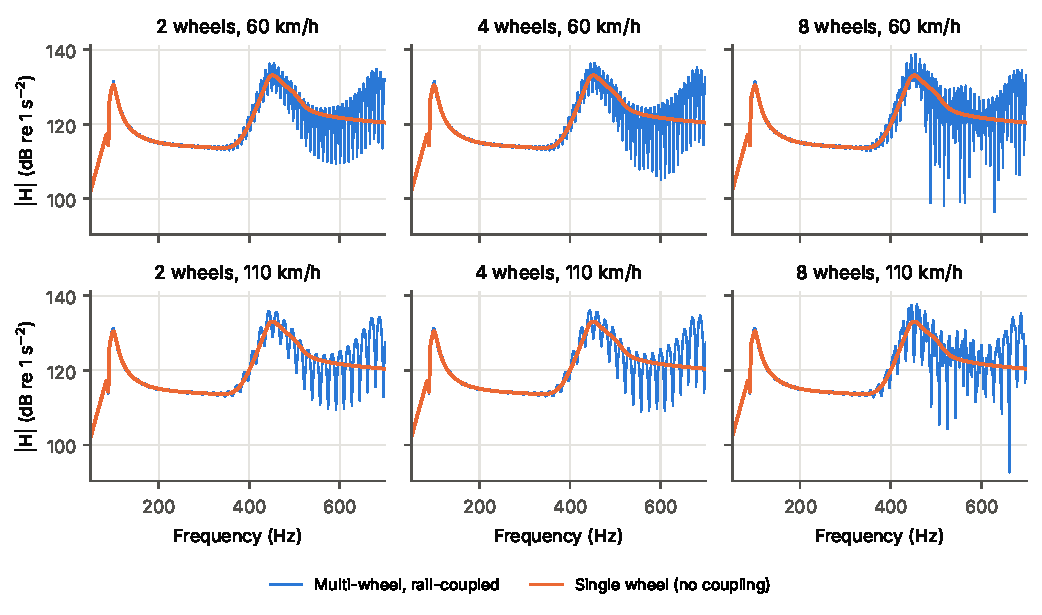
\includegraphics[width=\textwidth]{fig1_transfer_functions}
\caption{Axle-box acceleration per unit roughness, $|H|$, for 2, 4 and 8 rail-coupled wheels against
a single wheel without coupling, at 60 and 110~km/h. Data: \texttt{results/p2/fig1\_transfer.json}.}
\label{fig:transfer}
\end{figure}

\subsection{Verification}\label{sec:verification}
Table~\ref{tab:table2_verification} lists the checks of the reference model: free--free Timoshenko
frequencies against the closed form, the windowed energy balance of the steady-state solution,
frequency- against time-domain response, and mesh convergence. Unit tests cover the rail
receptance against Eq.~(11) of~\citep{carrigan2023} and the numerical inverse transform, and the
identity of the single-wheel coupled model with the rail-oscillator model.

% generated by experiments/make_tables.py from config/params.yaml, config/track.yaml; do not edit
\begin{table}[tbp]\centering\scriptsize
\caption{Model parameters and sources}\label{tab:table1_parameters}
\resizebox{\textwidth}{!}{\begin{minipage}{1.6\textwidth}\centering
\begin{tabular}{lllll}
\toprule
Group & Parameter & Value & Unit & Source \\ \midrule
Material & E & 2.10e11 & Pa & doc \S{}16 (standard steel) \\
Material & nu & 0.3 & - & doc \S{}16 \\
Material & rho & 7850 & kg/m\textasciicircum{}3 & doc \S{}16 \\
Axle & length & 2.18 & m & placeholder: typical standard-gauge freight axle \\
Axle & sections [outer $\xi$, d] & [[0.64,0.175],[0.86,0.2],[0.9,0.16],[1.09,0.13]] & m & placeholder: body / wheel seat / dust-guard collar / journal, typical EN 13103-type proportions \\
Axle & wheel\_xi & 0.75 & m & placeholder: contact plane \textasciitilde{} half of 1.5 m contact-point spacing \\
Axle & journal\_xi & 0.995 & m & placeholder: mid-journal bearing centre \\
Axle & n\_elements & 32 & - & brief: 20-40 elements; convergence checked at 20/30/40 \\
Axle & damping\_zeta & 0.01 & - & placeholder: 1\% stiffness-proportional at f\_ref \\
Axle & damping\_fref & 80 & Hz & placeholder: typical first wheelset bending frequency \\
Wheel & mass & 350 & kg & placeholder: 920 mm freight wheel \\
Wheel & diametral\_inertia & 20 & kg m\textasciicircum{}2 & placeholder: disc estimate m r\textasciicircum{}2/4 with rim correction \\
Wheel & r0 & 0.4575 & m & doc \S{}13 (new 915 mm wheel) \\
Bearing & kB0 & 1.0e9 & N/m & placeholder: tapered roller unit radial stiffness, order 1e8-1e9 \\
Bearing & cB & 5.0e3 & N s/m & placeholder: EHL/structural damping \\
Bearing & load\_exponent & 0.1 & - & doc Eq. (12): Q \textasciitilde{} delta\textasciicircum{}(10/9) gives k \textasciitilde{} Q\textasciicircum{}(1/10) \\
Axlebox & mass & 60 & kg & placeholder: housing + outer ring + adapter \\
Primary & kp & 1.0e6 & N/m & placeholder: freight primary vertical stiffness per axlebox \\
Primary & cp & 1.0e4 & N s/m & placeholder: equivalent linear damping per axlebox \\
Payload & W\_min & 5.5 & t & placeholder: empty freight wagon axle load \\
Payload & W\_max & 22.5 & t & placeholder: loaded (22.5 t axle load class) \\
Payload & W0 & 22.5 & t & reference load for kB0 (loaded) \\
Rail BS113A & A & 0.00717 & m\textasciicircum{}2 & CT23 Table 1 \\
Rail BS113A & rho & 7850 & kg/m\textasciicircum{}3 & CT23 Table 1 \\
Rail BS113A & E & 207.0e9 & Pa & CT23 Table 1 \\
Rail BS113A & I & 2.35e-05 & m\textasciicircum{}4 & CT23 Table 1 \\
Rail BS113A & G & 81.0e9 & Pa & CT23 Table 1 \\
Rail BS113A & kappa & 0.34 & - & CT23 Table 1 \\
Rail 60E1 & A & 0.00767 & m\textasciicircum{}2 & verify: EN 13674-1 60E1 section area 76.70 cm\textasciicircum{}2 (quoted from memory) \\
Rail 60E1 & I & 3.038e-05 & m\textasciicircum{}4 & verify: EN 13674-1 60E1 vertical-bending I\_x 3038.3 cm\textasciicircum{}4 (quoted from memory) \\
Foundation & standard\_kf\_lab & 154.0e6 & N/m\textasciicircum{}2 & CT23 Sec. 5.1.1: \textasciitilde{}100 MN/m per fastener (lab, Thompson et al.) at 0.65 m spacing \\
Foundation & resilient\_kf & 7.7e6 & N/m\textasciicircum{}2 & CT23 Sec. 5.1.1 (pass-by rail deflection, Cox \& Wang) \\
Foundation & eta\_f & 0.2 & - & CT23 Table 1 / Sec. 5.1.1 (literature range 0.2-0.3) \\
Contact & C\_H & 89.0e9 & N/m\textasciicircum{}1.5 & CT23 Sec. 5.1.2 citing Sanchis et al. (metro wheel/rail radii; freight wheel and 60E1 head radii differ: verify) \\
Layout & positions & [0.0,2.05,6.52,8.57,16.62,18.67,23.14,25.19,33.24,35.29,39.76,41.81] & m & CT23 Sec. 5.1.3 / Fig. 5: axle spacing 2.05, bogie centres 10.10 within a car, 6.52 across a coupling (positions derived from these) \\
\bottomrule
\end{tabular}

\par\smallskip{\footnotesize 15 of 35 entries are placeholders. Vehicle masses (wheel, axlebox, unsprung) stay placeholders until the target vehicle is confirmed; values marked 'verify' are to be checked against the cited standard.}
\end{minipage}}
\end{table}

% generated by experiments/make_tables.py from results/p1/verification.json, results/gates/G1.json; do not edit
\begin{table}[tbp]\centering\scriptsize
\caption{Verification of the reference model}\label{tab:table2_verification}
\resizebox{\textwidth}{!}{\begin{minipage}{1.6\textwidth}\centering
\begin{tabular}{llll}
\toprule
Check & Measured & Threshold & Gate \\ \midrule
Free--free Timoshenko frequencies vs closed form (max rel. error, 4 modes) & 3.62e-03 & 5e-03 & PASS \\
Energy balance, windowed integral (max rel. residual, 3 cases) & 1.3e-11 & 1e-06 & PASS \\
Frequency vs time domain, axlebox accel. (max rel. L2, 3 cases) & 1.8e-06 & 1e-03 & PASS \\
Mesh 20 vs 40 elements, modes (max rel. diff.) & 2.0e-03 & -- & -- \\
Gyroscopic neglect, $\Omega$/$\omega$$_1$ & 0.106 & -- & -- \\
\bottomrule
\end{tabular}

\par\smallskip{\footnotesize Rail receptance vs CT23 Eq. 11 and the numerical inverse transform, and the single-wheel coupling identity (1e-9), are unit tests in tests/test\_track.py (all pass).}
\end{minipage}}
\end{table}


% Section 3: method. Numbers: generated/numbers.tex.
\section{Estimation method}\label{sec:method}

\subsection{Observation model}\label{sec:obs}
Pass $i$ is a record of vertical axle-box acceleration over \NumRevs{} wheel revolutions, so its
length is fixed in space, $L = \NumRevs\cdot 2\pi r_0$, and its duration $T_i = L/V_i$ depends on the
pass speed $V_i$. The DFT coefficient $c_{ik}$ at bin $k$ belongs to the frequency $f_{ik} = k/T_i$
and to the same wavenumber $\gamma_k = 2\pi k/L$ on every pass. The analysis band is fixed in
frequency.

Rail roughness is a stationary Gaussian process with one-sided wavenumber spectrum
\begin{equation}
  G(\gamma) = G_\mathrm{ISO}(\gamma)\,g_{s(\gamma)},
\end{equation}
where $G_\mathrm{ISO}$ has the shape of the ISO~3095 limit spectrum~\citep{iso3095} and
$g_s$ is a free level in sub-band $s$, with $K$ sub-bands per one-third octave. The levels are
nuisance parameters: the method never measures roughness. The axle load of each pass, $W_i$, is a
nuisance with a Gaussian prior on $\log W_i$ centred on a weigh-in-motion reading with standard
deviation \WIMsigmaPct\%. The sensor noise is white with level $e_i$, estimated from an
out-of-band part of the same record. The globals $\bm\theta$ are the health parameters
$(k_{B0}, c_B)$, optionally with track parameters such as $k_f$ and $k_{H0}$.

Under this model the coefficients are approximately independent complex Gaussians with variance
\begin{equation}
  v_{ik} = |H(f_{ik};\bm\theta, W_i, V_i)|^2\, 2G(\gamma_k)\,\Delta\gamma + e_i,
  \label{eq:binvar}
\end{equation}
and the negative log-likelihood over $N$ passes is the multi-pass Whittle form~\citep{whittle1953}
\begin{equation}
  \ell(\bm\theta, \bm g, \bm W) = \sum_{i=1}^{N}\sum_k\left[\log v_{ik} + \frac{|c_{ik}|^2}{v_{ik}}\right]
  + \sum_{i=1}^{N}\frac{(\log W_i - \log\hat W_i)^2}{2\sigma_W^2}.
  \label{eq:whittle}
\end{equation}
The same structure, with the modal-force spectrum per band as the nuisance, underlies Bayesian
FFT operational modal analysis~\citep{au2011}.

\paragraph{Why speed diversity identifies the support.} Roughness is fixed in wavenumber, while the
resonance of the axlebox on its support is fixed in frequency. A pass at speed $V_i$ maps
wavenumber $\gamma$ to frequency $V_i\gamma/2\pi$, so passes at different speeds see the same
roughness sub-band through different parts of $|H|^2$. With a single speed, a change of $|H|^2$ and
a change of roughness level are indistinguishable sub-band by sub-band; with a spread of speeds
they separate. Figure~\ref{fig:crb-speed} shows the Cram\'er--Rao bound of $k_{B0}$ falling with
the speed spread for several sub-band resolutions $K$.

\begin{figure}[tbp]\centering
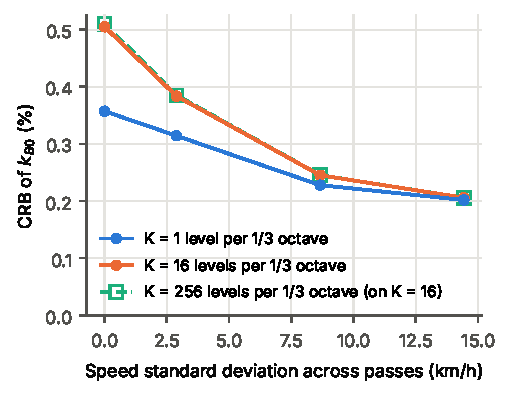
\includegraphics[width=0.55\textwidth]{fig2_crb_vs_speed_spread}
\caption{Effect of speed spread on identifiability. Cram\'er--Rao bound of $k_{B0}$ against the speed spread across passes, for $K$ roughness
levels per one-third octave ($N=50$, 40~dB, payload spread). Data:
\texttt{results/p1/bound\_speed\_subband.json}.}
\label{fig:crb-speed}
\end{figure}

\subsection{Debiased likelihood for multi-wheel cross terms}\label{sec:debias}
Equation~\eqref{eq:binvar} samples $|H|^2G$ at the bin. The expected periodogram of a finite
record is instead the spectrum convolved with the Fej\'er kernel $T\,\mathrm{sinc}^2((f-f_k)T)$.
The two agree when the spectrum is smooth on the scale of one bin, as for a single wheelset. They
do not agree once the multi-wheel phase factors in~\eqref{eq:H} put ripples of period $V/(d_k-d_j)$
close to the bin width. Following Sykulski et al.~\citep{sykulski2019}, we keep the Whittle form but
replace $v_{ik}$ by the exact expected periodogram,
\begin{equation}
  v_{ik} = \sum_m \frac{\mathrm{sinc}^2\!\big((f_m - f_{ik})T_i\big)}{M}\,
           |H(f_m)|^2\,2G(\gamma_m)\,\Delta\gamma + e_i,
  \label{eq:debiased}
\end{equation}
with the sum over a grid $M=\KernelFine$ times finer than the bins, truncated at $\pm\KernelHalfWidth$ bins
(a narrower truncation at $\pm30$ bins leaves a measurable bias; Section~\ref{sec:res-bias}). On the
simulated 12-wheel setup of~\citep{carrigan2023}, the bin-sampled model differs from the mean of
\DebiasRecords{} periodograms by an rms log-ratio of \DebiasBin{}; the debiased model differs by
\DebiasDeb{}, against \DebiasNoise{} expected from sampling alone (Fig.~\ref{fig:debias}).

\begin{figure}[tbp]\centering
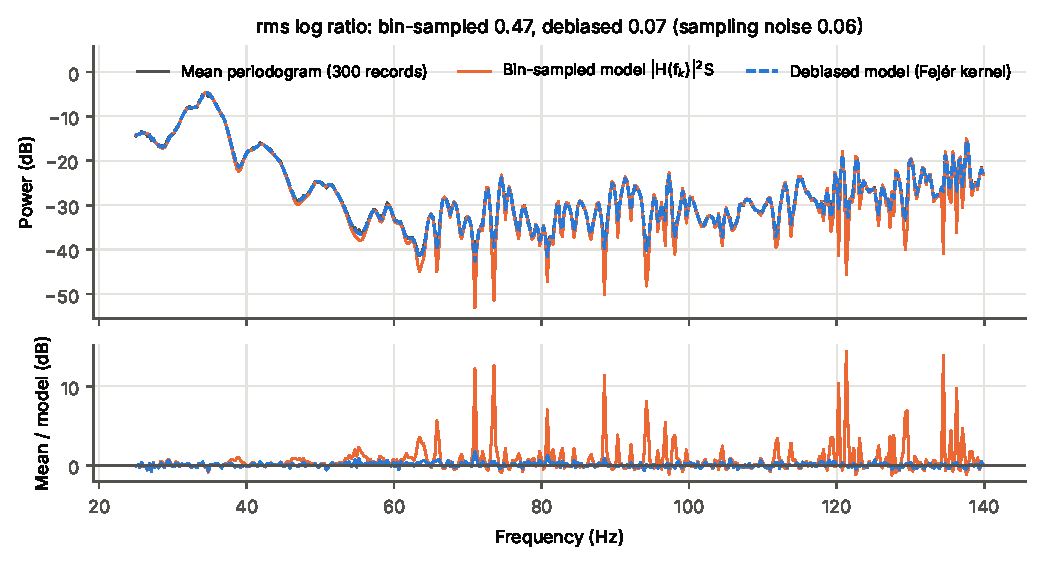
\includegraphics[width=\textwidth]{fig3_debiased_periodogram}
\caption{Check of the debiased likelihood. Mean periodogram of \DebiasRecords{} records against the bin-sampled and the debiased
(Fej\'er-convolved) models (top) and their ratio (bottom). Data:
\texttt{results/p2/debias\_check.json}.}
\label{fig:debias}
\end{figure}

\subsection{Profiling and optimisation}\label{sec:profile}
For given globals $\bm\theta$, the nuisances $(\log\bm g, \log\bm W)$ are profiled out by Fisher
scoring, warm-started from the previous evaluation. The globals are then found by Nelder--Mead on
the profile likelihood. With the debiased variance~\eqref{eq:debiased} the kernel mixes
neighbouring roughness sub-bands. The default scoring step attributes each bin's variance to its
own sub-band; the exact step uses the full derivative $\partial v_{ik}/\partial\log g_s$ over all
sub-bands and the corresponding Fisher matrix, so that its fixed point is the exact profile maximum.
Section~\ref{sec:res-bias} compares the two.

The transfer functions are computed directly from the finite-element and rail models (no
surrogate): a table of the coupled components $G_k(f;\bm\theta,W)$ over payload nodes, built from an
exact modal decomposition of the wheelset for each trial $\bm\theta$, is interpolated in $\log W$
and frequency.

\subsection{Uncertainty}\label{sec:uncertainty}
Wald intervals use the observed information of the profile likelihood (numerical Hessian).
Profile-likelihood intervals use the $\chi^2_1$ cut, re-optimising the other globals and all
nuisances. The Cram\'er--Rao bound (CRB) is the inverse expected Fisher information with every
nuisance free and the weigh-in-motion prior included. When records repeat over the same section,
the independence assumed in~\eqref{eq:whittle} fails across passes; the variance is then taken
from a sandwich estimator clustered on DFT bin (the same wavenumber on every pass).
Where the Wald intervals under-cover in simulation (Section~\ref{sec:res-headline}), they are
simulation-calibrated for the design: the mean bias of $\log\hat k_{B0}$ found by simulation is
subtracted and the standard error is multiplied by the simulated ratio of RMSE to standard error,
checked on held-out simulation seeds.

\subsection{Relative change and detection}\label{sec:relative}
The monitoring output is the change of support stiffness between a baseline period and a later
period of the same vehicle and sensor, each with $N$ passes in the same payload band. Two bands are used:
empty (axle load 5.5--7~t) and laden (20--22.5~t); in each, the estimator uses the band's primary
stiffness and damping (Table~\ref{tab:table1_parameters}), and the weigh-in-motion payload assigns each
pass to its band. Pooling passes over the whole payload range requires a payload-dependent model of the
primary suspension (Section~\ref{sec:res-primary}). The change is

\begin{equation}
  D = \log\hat k_{B0}^{\,\mathrm{later}} - \log\hat k_{B0}^{\,\mathrm{base}},
\end{equation}
reported as $\Delta k_{B0}/k_{B0} = \exp(D)-1$. A misspecified model parameter biases $\log\hat k_{B0}$
in both periods; to first order the common part cancels, and the remainder scales with the change
itself. We therefore use the interval
\begin{equation}
  D \pm 1.645\sqrt{\mathrm{se}_\mathrm{base}^2 + \mathrm{se}_\mathrm{later}^2 + (\kappa D)^2},
  \label{eq:interval}
\end{equation}
where $\kappa$ is the model-form gain uncertainty: the root sum of squares, over the uncertain model
parameters, of the gain $\partial(\hat D/D)/\partial\log(\text{parameter})$ times that parameter's
$1\sigma$ log range. Foundation stiffness can drift between periods (seasonal pad stiffness), so the
default fit re-estimates $k_f$ and $k_{H0}$ in each period together with $(k_{B0}, c_B)$.

A loss is declared when $D < -1.645\,s_0$, where $s_0$ is the standard deviation of $D$ with no
change (5\% false-alarm rate, one-sided). The minimum detectable change (MDC) is the true decrease
detected with probability 0.9, $\mathrm{MDC} = (1.645 + 1.282)\,s_0$ without bias; with a bias in
$D$ it is found by interpolating the bias against the true change.

\subsection{Model-form bias}\label{sec:pseudotrue}
The large-sample bias under a misspecified model is the pseudo-true parameter: the minimiser of the
expected value of~\eqref{eq:whittle} when the periodograms are replaced by their expectations under
the true model. It is computed by the same profiled fit with $|c_{ik}|^2$ replaced by the true
$v_{ik}$, and was checked against full Monte Carlo fits. A first-order (score) approximation was
found to fail for large parameter errors and is not used.

\subsection{Implementation and use of AI}\label{sec:implementation}
The simulation and estimation code was developed with the assistance of an AI coding tool, Claude Code
(developer: Anthropic; model: Claude Opus 5.5). It was used to write the code (the finite-element and
rail models, the simulation and estimation scripts, and the scripts that generate tables, figures and
the numbers quoted in the text) and to assist the literature search. All code was reviewed, tested and
verified by the authors: unit tests cover the finite-element and rail models, the model is verified
against closed-form solutions (Table~\ref{tab:table2_verification}), and every result in this paper is
regenerated by script from stored, version-controlled result files.

% Section 4: results. Placeholders until the current runs finish; tables will be \input from
% ../results/tables/ and numbers from generated/numbers.tex.
\section{Results}\label{sec:results}
\subsection{Headline Monte Carlo on the rail-coupled model}\label{sec:res-headline}
\placeholder{Table 3 (results/p2/headline\_mw.json).}
\subsection{Speed spread and number of passes}\label{sec:res-speed}
\placeholder{Table 4.}
\subsection{Multi-wheel coupling}\label{sec:res-multiwheel}
\placeholder{Table 5, Fig. 4.}
\subsection{Estimator bias diagnosis}\label{sec:res-bias}
\placeholder{results/p3/validation\_mc.json, bias\_diag.}
\subsection{Model-form sensitivity}\label{sec:res-modelform}
\placeholder{Fig. 5, Table 6.}
\subsection{Relative change, interval and detection}\label{sec:res-relative}
\placeholder{Fig. 6, Tables 7--8; $\kappa$ revalidation (results/p3/validation\_mc.json).}
\subsection{Health relevance and the load exponent}\label{sec:res-exponent}
\placeholder{results/p3/bearing\_clearance.json, results/p3/exponent\_bound.json.}
\subsection{Foundation drift}\label{sec:res-drift}
\placeholder{Table 11; drift Monte Carlo at $k_f\times0.8$.}
\subsection{Wheel roughness at rotation orders}\label{sec:res-wheel}
\placeholder{Table 9.}
\subsection{Repeated passes over one section}\label{sec:res-repeated}
\placeholder{Table 10.}
\subsection{Validation against the P2 failure mode}\label{sec:res-p2}
\placeholder{Fig. 7, Table 12.}

% Section 5: discussion. Numbers: generated/numbers.tex.
\section{Discussion}\label{sec:discussion}
\placeholder{Section 5 body after Section 4 is final.}

\subsection{Limitations}\label{sec:limitations}
\paragraph{Load exponent as a clearance indicator.} Clearance growth changes not only the level of the
effective support stiffness but also its dependence on axle load, because a larger clearance shrinks
the load zone more at light load. In principle the load exponent $p$ of~\eqref{eq:powerlaw} could
therefore separate clearance growth from other losses of support stiffness. With the exponent free
alongside $(k_{B0}, c_B)$ and payloads spanning \PayloadMin--\PayloadMax~t, the Cram\'er--Rao bound of
$p$ is \ExpCRBFifty{} for $N = 50$ passes and \ExpCRBTwoHundred{} for $N = 200$, and freeing $p$ raises
the bound of $k_{B0}$ from \KBCRBExpFixed\% to \KBCRBExpFree\% ($N=50$). Under the series reading of
the support (placeholder bearing geometry), 10 and 20~\textmu m of clearance growth raise the
effective exponent by only \ExpShiftTen{} and \ExpShiftTwenty{}. Detecting a shift between two
periods (one-sided 5\% false alarm, 90\% detection) needs \ExpMDCFifty{} at $N=50$ and
\ExpMDCTwoHundred{} at $N=200$, so only 20~\textmu m at $N=200$ would be detected. The exponent is
therefore held fixed in the estimator, and the method reports a loss of effective support stiffness
without attributing it to a mechanism.

% Section 6: conclusions. Numbers: generated/numbers.tex.
\section{Conclusions}\label{sec:conclusions}
The vertical support stiffness of a wheelset bearing can be identified from in-service axle-box
acceleration without measuring the rail roughness, by pooling passes at different speeds and payloads
in a debiased Whittle likelihood in which the roughness levels are free nuisance parameters. For a
representative freight wagon on ballasted track, simulations show that:
\begin{itemize}
\item with 50 passes at 60--110~km/h the support stiffness is estimated with a bias of
  \HLTwentyBias--\HLFortyBias\% and a root-mean-square error of \HLTwentyRMSE--\HLFortyRMSE\%, close to
  the Cram\'er--Rao bound at 20~dB and \HLFortyRatioCRB{} times it at 40~dB, where intervals are
  calibrated by simulation;
\item the speed spread is the design variable that makes the support stiffness identifiable, and the
  wheel-to-wheel coupling through the rail must be modelled, since ignoring it biases the estimate by
  \IgnoreCouplingForty\%;
\item the absolute level carries a model-form uncertainty of about \BudgetCoest\%, so the method is a
  trend monitor: re-estimating the foundation and contact stiffness in each period, a decrease of
  \MDCCalFiftyTwenty--\MDCCalFiftyForty\% is detectable with 50 passes per period, and a 20\% change of
  the foundation raises \DriftMCCoestFA{} false alarm in \DriftMCCoestN{} trials;
\item a loss of housing, adapter or pad stiffness reaches the identified stiffness directly, while
  clearance growth is diluted by the stiff roller contacts, so the method reports support-stiffness
  loss without attributing it to a mechanism.
\end{itemize}
The next steps are a field test with a controlled change of support stiffness; application to
freight wagons of Indian Railways, once vehicle-specific values are available from RDSO; an extension of
the model to the pinned--pinned frequency band; and calibrated intervals for the track-side use of the
same likelihood.


% Statements required by the MSSP Guide for Authors, in the required order, before the references.

\section*{CRediT authorship contribution statement}
% One line per author with the CRediT roles (https://credit.niso.org/); to be completed by the authors.
\textbf{[Given name 1] [Family name 1]:} [Conceptualization, Methodology, Software, Validation, Formal
analysis, Investigation, Writing -- original draft, Writing -- review \& editing, Visualization].
\textbf{[Given name 2] [Family name 2]:} [roles].

\section*{Declaration of competing interest}
% Must match the text entered in the Elsevier declarations tool.
[The authors declare that they have no known competing financial interests or personal relationships
that could have appeared to influence the work reported in this paper.]

\section*{Funding}
This research did not receive any specific grant from funding agencies in the public, commercial, or
not-for-profit sectors.

\section*{Data availability}
The code that generates every result, table, figure and number in this paper, and the stored result
files, are available at \url{https://github.com/Shreyansh369/wheelset-s2pinn} and archived at Zenodo
(\url{https://doi.org/[ZENODO DOI]}). All data are simulated; no measured data were used. The repository
references the third-party S$^2$-PINN code of Li and Onwunta~\citep{li2026s2pinn} as a pinned external
dependency; that code is not redistributed.

\section*{Acknowledgements}
[To be completed by the authors.]

\section*{Declaration of generative AI and AI-assisted technologies in the manuscript preparation process}
During the preparation of this work, the authors used Claude Code (Anthropic) in order to develop the
simulation and estimation code, assist the literature search, and draft and edit the manuscript text.
After using this tool/service, the authors reviewed and edited the content as needed and take full
responsibility for the content of the published article.


\bibliographystyle{elsarticle-num}
\bibliography{refs}
\end{document}
